% Apêndice A: endereçamento aberto com sondagem linear (m = 7) e a marca de removido.
\documentclass[border=4pt]{standalone}
\usepackage[utf8]{inputenc}
\usepackage[T1]{fontenc}
% Estilo comum das figuras de vetores (capítulo 8).
\usepackage{tikz}
\usetikzlibrary{arrows.meta, positioning, calc, decorations.pathreplacing}
\definecolor{navy}{RGB}{23,45,80}
\definecolor{laranja}{RGB}{250,110,29}
\definecolor{cinzalogo}{RGB}{107,114,126}
\definecolor{azul}{RGB}{205,222,247}
\tikzset{
  casa/.style={draw=navy, line width=0.9pt, minimum width=8mm, minimum height=7mm,
               inner sep=0pt, font=\sffamily\small},
  pronta/.style={casa, fill=azul},
  parte/.style={casa, fill=laranja!12},
  marcada/.style={casa, fill=laranja!45, draw=laranja},
  fora/.style={casa, draw=cinzalogo!60, dashed, fill=white, text=cinzalogo!60},
  indice/.style={font=\sffamily\scriptsize, text=cinzalogo},
  explica/.style={font=\sffamily\small, text=navy, anchor=east},
  legenda/.style={font=\sffamily\scriptsize, text=cinzalogo},
  rotulo/.style={font=\sffamily\small\bfseries, text=navy},
  seta/.style={-{Stealth[length=2.2mm]}, navy, line width=0.9pt},
  chave/.style={decorate, decoration={brace, amplitude=4pt, mirror}, navy, line width=0.8pt},
}
% \vetor{nome}{x}{y}{valor/estilo, valor/estilo, ...}: casas lado a lado, chamadas nome0, nome1...
\newcommand{\vetor}[4]{%
  \foreach \valor/\estilo [count=\i from 0] in {#4} {
    \node[\estilo] (#1\i) at ($(#2, #3) + (\i*0.8, 0)$) {\valor};
  }
}

\tikzset{
  removida/.style={casa, fill=cinzalogo!20, text=cinzalogo, font=\sffamily\scriptsize},
}
\begin{document}
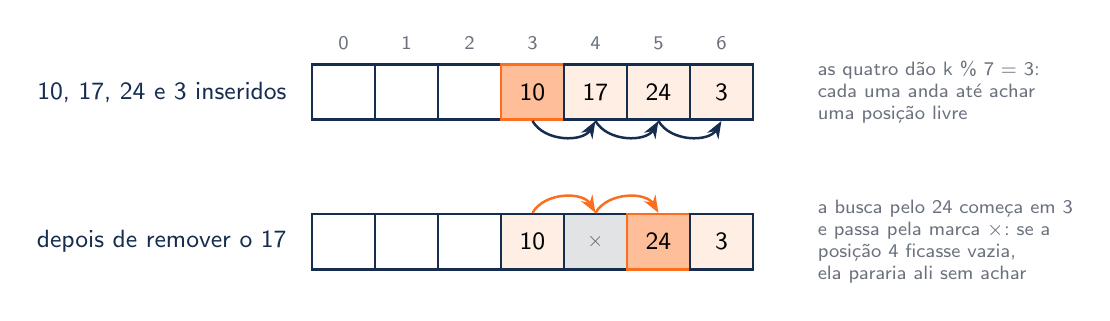
\begin{tikzpicture}
  \node[explica] at (-0.6, 0) {10, 17, 24 e 3 inseridos};
  \vetor{a}{0}{0}{/casa, /casa, /casa, 10/marcada, 17/parte, 24/parte, 3/parte}
  \foreach \i in {0,...,6} { \node[indice, above=0.5mm of a\i] {\i}; }
  \foreach \i/\j in {3/4, 4/5, 5/6} {
    \draw[seta] (a\i.south) to[out=-60, in=-120] (a\j.south);
  }
  \node[legenda, align=left, anchor=west] at (5.9, 0)
    {as quatro dão k \% 7 = 3:\\cada uma anda até achar\\uma posição livre};

  \node[explica] at (-0.6, -1.9) {depois de remover o 17};
  \vetor{b}{0}{-1.9}{/casa, /casa, /casa, 10/parte, {\texttimes}/removida, 24/marcada, 3/parte}
  \draw[seta, laranja] (b3.north) to[out=60, in=120] (b4.north);
  \draw[seta, laranja] (b4.north) to[out=60, in=120] (b5.north);
  \node[legenda, align=left, anchor=west] at (5.9, -1.9)
    {a busca pelo 24 começa em 3\\e passa pela marca \texttimes: se a\\posição 4 ficasse vazia,\\ela pararia ali sem achar};
\end{tikzpicture}
\end{document}
